\documentclass{article}

\usepackage{amssymb, amsmath}
\usepackage{listings}
\usepackage[usenames,dvipsnames]{color}
\usepackage{courier}
\usepackage{parskip}
\usepackage{graphicx}
\usepackage{float}
\usepackage{listings}

\lstset{ %
  backgroundcolor=\color{White},   % choose the background color
  basicstyle=\ttfamily,        % size of fonts used for the code
  breaklines=true,                 % automatic line breaking only at whitespace
  captionpos=b,                    % sets the caption-position to bottom
  commentstyle=\color{mygreen},    % comment style
  escapeinside={\%*}{*)},          % if you want to add LaTeX within your code
  keywordstyle=\color{blue},       % keyword style
  stringstyle=\color{mymauve},     % string literal style
  frame = single
}

\definecolor{mygreen}{rgb}{0,0.6,0}
\definecolor{mygray}{rgb}{0.5,0.5,0.5}
\definecolor{mymauve}{rgb}{0.58,0,0.82}

\author{Verdu, J.-M., Fernandez, M. , Kreienkamp, T.}

\title{Text Mining Homework 4}

\begin{document}

\section{}


\subsection{}

For the main part of this exercise, please see our groups code.

After visualizing the \lstinline{tf_idf ranking}, we decide to use 8000 stems. 

\subsection{}

The following figures plot the perplexity scores as a function of the samples we draw.

\begin{figure}[H]
\centering
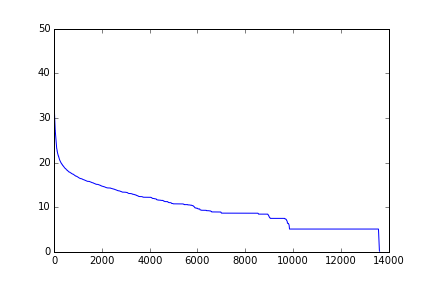
\includegraphics[width=120mm]{tfidf_ranking.png}
\caption{TF-IDF Ranking of Stems}
\end{figure}

\subsection{}

The following figures plot the perplexity scores as a function of the samples we draw.

\begin{figure}[H]
\centering
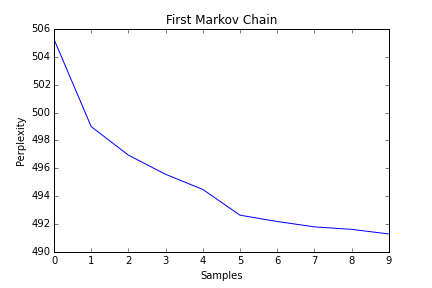
\includegraphics[width=120mm]{firstchain.png}
\end{figure}

\begin{figure}[H]
\centering
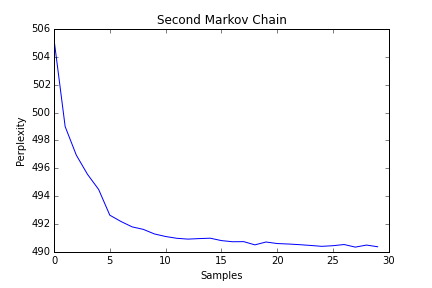
\includegraphics[width=120mm]{secondchain.png}
\end{figure}

\begin{figure}[H]
\centering
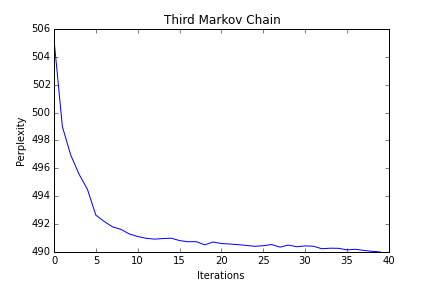
\includegraphics[width=120mm]{thirdchain.png}
\end{figure}

We see that they stabilize at about the last 20 draws in the third markov chain. Since the exercise text restricts us to ten, we choose to keep the last ten samples. 
After having generatied the topics and document-topic distributions (see code), let's examine the topics. 

\begin{lstlisting}
topic0,oper,financ,support,econom,countri,region,project,agreement,cooper,provis
topic1,eupol,copp,rafah,head,action,bam,oper,polic,staff,eusr
topic2,product,materi,origin,use,ex,manufactur,work,valu,declar,head
topic3,budget,payment,research,commit,programm,amount,revenu,titl,financi,will
topic4,remarksthi,reserv,basiscouncil,year,action,third,basisregul,servic,project,train
topic5,commit,expenditur,payment,programm,area,polici,appropri,chapter,action,countri
topic6,appropri,financi,revenu,year,remark,chapter,expenditur,staff,assign,servic
topic7,agreement,price,flower,rose,carnat,protocol,origin,fix,strip,bank
topic8,al,birth,syrian,regim,syria,minist,repress,respons,civilian,popul
topic9,appropri,outturn,payment,differenti,commit,financi,expenditur,research,legal,programm
topic10,fund,parliament,project,pilot,innov,payment,commit,remark,programm,financi
topic11,al,born,takfir,hijra,card,ident,activist,algier,aka,hofstadgroep
topic12,row,part,credit,crr,exposur,asset,amount,financi,institut,column
topic13,syn,var,product,brassica,leav,remov,bean,citru,seed,root
topic14,bio,third,product,countri,number,code,categori,point,permit,month
\end{lstlisting}


Here we see some interesting patterns. For example, topic11 seems to be a djihadism-terrorism related topic (since it talks about the hofstadgroep, a Dutch terrorist organization influenced by Takfir wal-Hijra), wereas topic1 might be related to police, and topic6 is definitely economy-related. 

\subsection{}

To generate out of sample distributions, we use the titles of our data set. 

We think that it would be interesting to see if the estimated topic of documents and titles match. This is the case for 69.6\% of the documents. This sounds reasonable at first. Looking at the histograms of documents (first) and titles (second) we see that the picture is quite different.. This is probably due to the short length of the titles which makes it a lot harder to do valid inference on them. 

\begin{figure}[H]
\centering
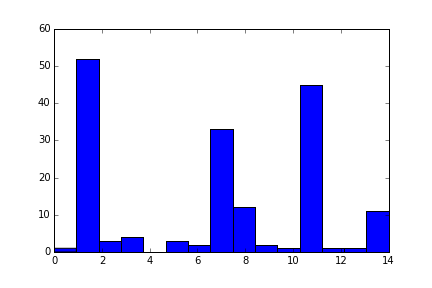
\includegraphics[width=120mm]{doctopicshist.png}
\end{figure}

\begin{figure}[H]
\centering
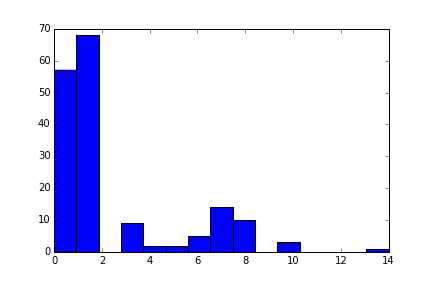
\includegraphics[width=120mm]{titletopicshist.png}
\end{figure}

\subsection{}

We spot check documents 1 and 2 (0 and 1 in Python Indexing) which match their topic (1) (police / border control missions). 6 and 7,  also belonging to the same topic (7) seem also to talk about a similar topic, regarding import / customs regulations. Thus, we are quite satisfied with the topic selections.





\end{document}